% Created 2013-09-08 Sun 15:53
\documentclass[11pt]{article}
\usepackage[utf8]{inputenc}
\usepackage[T1]{fontenc}
\usepackage{fixltx2e}
\usepackage{graphicx}
\usepackage{longtable}
\usepackage{float}
\usepackage{wrapfig}
\usepackage[normalem]{ulem}
\usepackage{textcomp}
\usepackage{marvosym}
\usepackage{wasysym}
\usepackage{latexsym}
\usepackage{amssymb}
\usepackage{amstext}
\usepackage{hyperref}
\tolerance=1000
\usepackage{tikz}
\usepackage{tikz}
\usepackage{tikz-cd}
\usetikzlibrary{matrix,arrows,positioning,scopes,chains}
\tikzset{node distance=2cm, auto}
\author{Brian Beckman}
\date{\today}
\title{Fluent, Composable Error Handling}
\hypersetup{
  pdfkeywords={},
  pdfsubject={},
  pdfcreator={Emacs 24.3.1 (Org mode 8.0.7)}}
\begin{document}

\maketitle
\tableofcontents


\section{Introduction}
\label{sec-1}

Consider a program composed of \emph{serially dependent computations},
any of which produces either a value to feed to the next computation
in-line, or an error. If any computation in the sequence produces an
error, no downstream computations should be attempted and that error
should be the result of the entire sequence.

We show a sequence of solutions of increasing elegance in Java and
Clojure for this program. The solutions are in fluent style, which
minimizes the number of temporary variables that must be invented
and named. This style directly mimics the abstract data flow of the
solution.

We further show techniques for fluent error handling, both with
exceptions and with returned error codes.
\section{Motivating Example Problem}
\label{sec-2}

As a concrete example, suppose we must
get an authorization token, do a database lookup, do a web-service
call, filter the results of that call, do another web-servie call,
and then combine the results. The data flow of our program
resembles that in figure \ref{fig:dataflow}.

\begin{figure}
\begin{center}
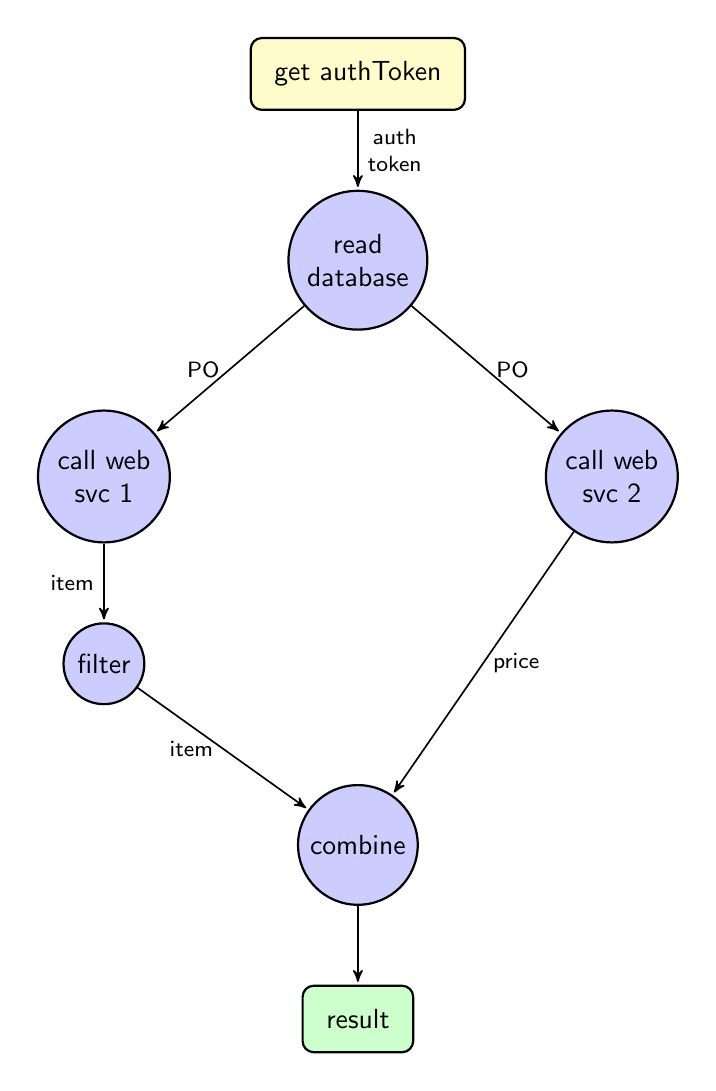
\begin{tikzpicture}[
  font=\sffamily,
  every matrix/.style={ampersand replacement=\&,column sep=1cm,row sep=1cm},
  source/.style={draw,thick,rounded corners,fill=yellow!20,inner sep=.3cm},
  process/.style={draw,thick,circle,fill=blue!20},
  sink/.style={source,fill=green!20},
  rectangle/.style={draw,very thick,shape=rectangle,inner sep=.3cm},
  dots/.style={gray,scale=2},
  invisible/.style={},
  to/.style={->,>=stealth',shorten >=1pt,semithick,font=\sffamily\footnotesize},
  every node/.style={align=center}]

  % Position  nodes using a matrix layout
  \matrix{
      {}
      \& \node[source] (auth) {get authToken};
      \& \\

      {}
      \& \node[process] (database) {read\\database};
      \& \\

      \node[process] (wscall1) {call web\\svc 1};
      \& 
      \& \node[process] (wscall2) {call web\\svc 2}; \\

      \node[process] (filter) {filter};
      \&
      \& \node[invisible] (placeholder) {}; \\

      {}
      \& \node[process] (combine) {combine};
      \& \\

      {}
      \& \node[sink] (result) {result};
      \& \\
  };

  % Draw the arrows between the nodes and label them.
  \draw[to] (auth) -- node[midway,right] {auth\\token} (database);
  \draw[to] (database) -- node[midway,left] {PO} (wscall1);
  \draw[to] (database) -- node[midway,right] {PO} (wscall2);
  \draw[to] (wscall1)  -- node[midway,left] {item} (filter);
  \draw[to] (filter)   -- node[midway,left] {item} (combine);
  \draw[to] (wscall2)  -- node[midway,right] {price} (combine);
  \draw[to] (combine)  -- (result);

\end{tikzpicture}
\end{center}
\caption{\label{fig:dataflow}Serially dependent computations}
\end{figure}

\subsection{Fluent Solution in Java, No Error Handling}
\label{sec-2-1}

In the \mbox{C++ -- like} languages, including JavaScript and Java,
we might keep intermediate results in instance variables and model
the flow as methods that produce instances from instances, that is,
as \textbf{transforms}. This style is called \textbf{fluent style}
because the text of the program resembles the flow in the diagram.

Imagine a \emph{main} program like the following, in which transforms are
on their own lines, indented from their \emph{sources} by one
\mbox{4-space} tab stop. The \textbf{source} of a transform is an
expression that produces an object to feed downstream.

\begin{verbatim}
public static void main(String[] args) {
    Computation databaseResults = new Computation()
        .authorize()
        .readDatabase();
    String result = databaseResults
        .callWebService()
        .filterResults()
        .combineResults(databaseResults
            .callOtherWebService());
    System.out.println(result); }
\end{verbatim}

Notice that we save the \emph{Computation} produced by reading the
database in its own local variable, namely \emph{databaseResults}. We do
so because the dataflow branches from that result and we need to
use it twice, once as the source for calling the first web service
and once as the source for calling the second web service. If not
for this branching and recombining of the dataflow, we might have
written the entire program as one, fluent expression with no
intermediate variables.

Also note the compressed style, minimizing blank lines and lines
with just one closing brace. We adopt this style to save space in
this 

The following is a complete program that mocks out the database and
web-service calls as static JSON objects encoded in strings, and can
be compiled and executed, even online in some sandbox like
\url{http://www.compileonline.com/compile_java_online.php}.

\begin{verbatim}
public class Computation {
    private String authToken;
    private String databaseResults;
    private String webServiceCallResults;
    private String filteredWebServiceCallResults;
    private String otherWebServiceCallResults;

    public Computation () {}
    public Computation authorize() {
        authToken = "John's credentials";
        return this; }
    public Computation readDatabase() {
        databaseResults = "{\"name\":\"John\", \"PO\":\"421357\"}";
        return this; }
    public Computation callWebService() {
        webServiceCallResults =
            "[{\"item\":\"camera\"}, {\"item\":\"shoes\"}]";
        return this; }
    public Computation filterResults() {
        filteredWebServiceCallResults =
            "[{\"item\":\"camera\"}]";
        return this; }
    public Computation callOtherWebService() {
        otherWebServiceCallResults = "{\"price\":\"420.00\"}";
        return this; }
    public String combineResults(Computation other) {
        return "{[" + filteredWebServiceCallResults +
            "," + otherWebServiceCallResults + "]}"; }

    public static void main(String[] args) {
        Computation databaseResults = new Computation()
            .authorize()
            .readDatabase();
        String result = databaseResults
            .callWebService()
            .filterResults()
            .combineResults(databaseResults
                .callOtherWebService());
        System.out.println(result);
}   }
\end{verbatim}
\subsection{Fluent Solution in Java, with Exceptions}
\label{sec-2-2}

The program above has \emph{no} error handling. At this point, let us
agree that we \emph{must} have error handling in all but academic toys.

One of the better techniques for error handling in fluent style is
with exceptions. If each sub-computation is responsible for
throwing its own exception with error details, then a single
try-catch suffices to get error details out of the overall
sequence, leaving the essential dataflow expression unchanged. Our
main routine has minimal changes, and becomes simply

\begin{verbatim}
public static void main(String[] args) {
    try {
        Computation databaseResults = new Computation()
            .authorize()
            .readDatabase();
        String result = databaseResults
            .callWebService()
            .filterResults()
            .combineResults(databaseResults
                .callOtherWebService());
        System.out.println(result); }
    catch (Exception e) {
        System.out.println(e.getMessage());
}   }
\end{verbatim}
noting, in passing, that we ignore resource freeing (database
connections, sockets, file handles, etc.) in this
paper.\footnote{Idiomatically, resource management can be handled in a
   \emph{finally} clause or with Java 7's automatic resource management.
   See \url{http://bit.ly/15GYkMh}}

Let's give each mocked sub-computation a \mbox{10\%} chance of
erroring, and our entire sample becomes just the following:

\begin{verbatim}
import java.util.Random;
public class Computation {
    private String authToken;
    private String databaseResults;
    private String webServiceCallResults;
    private String filteredWebServiceCallResults;
    private String otherWebServiceCallResults;
    private static Random random = new java.util.Random();
    private static Boolean randomlyError() {
        return random.nextDouble() < 0.10; }

    public Computation () {}
    public Computation authorize() throws Exception {
        if (randomlyError()) { throw new Exception("auth errored"); }
        authToken = "John's credentials";
        return this; }
    public Computation readDatabase() throws Exception {
        if (randomlyError()) { throw new Exception("database errored"); }
        databaseResults = "{\"name\":\"John\", \"PO\":\"421357\"}";
        return this; }
    public Computation callWebService() throws Exception {
        if (randomlyError()) { throw new Exception("ws1 errored"); }
        webServiceCallResults =
            "[{\"item\":\"camera\"}, {\"item\":\"shoes\"}]";
        return this; }
    public Computation filterResults() throws Exception {
        if (randomlyError()) { throw new Exception("filter errored"); }
        filteredWebServiceCallResults =
            "[{\"item\":\"camera\"}]";
        return this; }
    public Computation callOtherWebService() throws Exception {
        if (randomlyError()) { throw new Exception("ws2 errored"); }
        otherWebServiceCallResults = "{\"price\":\"420.00\"}";
        return this; }
    public String combineResults(Computation other) throws Exception {
        if (randomlyError()) { throw new Exception("combine errored"); }
        return "{[" + filteredWebServiceCallResults +
            "," + otherWebServiceCallResults + "]}"; }

    public static void main(String[] args) {
        try {
            Computation databaseResults = new Computation()
                .authorize()
                .readDatabase();
            String result = databaseResults
                .callWebService()
                .filterResults()
                .combineResults(databaseResults
                    .callOtherWebService());
            System.out.println(result); }
        catch (Exception e) {
            System.out.println(e.getMessage());
}   }   }
\end{verbatim}
\subsection{Fluency Lost Without Exceptions}
\label{sec-2-3}

Error handling with exceptions is
debatable,\footnote{\url{http://www.joelonsoftware.com/items/2003/10/13.html}}
especially in Java, where runtime exceptions need not be
declared,\footnote{\url{http://bit.ly/1e5P6Cg}} but the alternative of checked
exceptions can be considered harmful.\footnote{\url{http://bit.ly/9NyrdD}}

Rather than join the debate, just imagine that we have decided
against exceptions for whatever reason and see if we can write
reasonable code.

Add a private \emph{String} field, \emph{errorResult}, and let every method
set the error result if and only if it errors. We must change
\emph{combineResults}; it can no longer return just a \emph{String}, but
rather a \emph{Computation}, because it may, itself, produce an error.
Furthermore, we lose the fluent style because every call must be
individually checked.

A particularly nasty way to do this is as follows:

\begin{verbatim}
public static String computation () {
    Computation c1 = new Computation();
    Computation c2 = c1.authorize();
    if (c2.errorResult.isEmpty()) {
        Computation c3 = c2.readDatabase();
        if (c3.errorResult.isEmpty()) {
            Computation c4 = c3.callWebService();
            if (c4.errorResult.isEmpty()) {
                Computation c5 = c4.filterResults();
                if (c5.errorResult.isEmpty()) {
                    Computation c6 = c3.callOtherWebService();
                    if (c6.errorResult.isEmpty()) {
                        Computation c7 = c5.combineResults(c6);
                        if (c7.errorResult.isEmpty()) {
                            return c7.getResult(); }
                        else {return c7.errorResult;} }
                    else {return c6.errorResult;} }
                else {return c5.errorResult;} }
            else {return c4.errorResult;} }
        else {return c3.errorResult;} }
    else {return c2.errorResult;} }
public static void main(String[] args) {
    System.out.println(computation()); }
\end{verbatim}

This is so intolerable as to barely deserve criticism, despite the
fact that its working set is optimized for the positive
path!\footnote{The error branches are all at addresses far from the
   common-case, non-error branches, which are clustered together for
   maximum locality.} We've lost any correspondence between the
program text and the program specification, and all options for
nesting and placement of curly braces are ludicrous. Changing the
computation graph would entail a sickening amount of work -- code
like this is best left to automatic code generators, if we
tolerate it at all.

The prevailing style, nowadays, is to reverse error branches and to
return as early as possible from the main routine. I have seen many
instances of this style in shipped code from pre-eminent shops.
Despite the fact that multiple returns were condemned in the dogma
of structured programming and are lethal in code that manages
resources,\footnote{\url{http://bit.ly/sAvDmY}} the justification for this is
three-fold:
\begin{itemize}
\item it results in linear code that can be read from top to bottom
\item edits to the computation graph entail just adding or subtracting
a localized block of a few lines of code and adjusting a few
temporary variables
\item modern compilers can reverse the branches in the generated code
automatically after a post-compilation profiling
step\footnote{\url{http://en.wikipedia.org/wiki/Profile-guided_optimization}}
\end{itemize}

This alternative\footnote{favored in the previously cited
   Joel-on-Software blog} is the following:

\begin{verbatim}
public static String computation() {
    Computation c1 = new Computation();
    Computation c2 = c1.authorize();
    if (! c2.errorResult.isEmpty()) {return c2.errorResult;}
    Computation c3 = c2.readDatabase();
    if (! c3.errorResult.isEmpty()) {return c3.errorResult;}
    Computation c4 = c3.callWebService();
    if (! c4.errorResult.isEmpty()) {return c4.errorResult;}
    Computation c5 = c4.filterResults();
    if (! c5.errorResult.isEmpty()) {return c5.errorResult;}
    Computation c6 = c3.callOtherWebService();
    if (! c6.errorResult.isEmpty()) {return c6.errorResult;}
    Computation c7 = c5.combineResults(c6);
    if (! c7.errorResult.isEmpty()) {return c7.errorResult;}
    return c7.getResult(); }
public static void main(String[] args) {
    System.out.println(computation()); }
\end{verbatim}

This, at least, gets rid of the ludicrous nesting, but exposes another
deep weakness: we have a proliferation of temporary variables just to
hold the \emph{Computations} returned by the intermediate stages. Why
bother with this when we have no hope of fluent style? Let's go to

\begin{verbatim}
public static String computation() {
    Computation c1 = new Computation();
    c1.authorize();
    if (! c1.errorResult.isEmpty()) {return c1.errorResult;}
    c1.readDatabase();
    if (! c1.errorResult.isEmpty()) {return c1.errorResult;}
    c1.callWebService();
    if (! c1.errorResult.isEmpty()) {return c1.errorResult;}
    c1.filterResults();
    if (! c1.errorResult.isEmpty()) {return c1.errorResult;}
    c1.callOtherWebService();
    if (! c1.errorResult.isEmpty()) {return c1.errorResult;}
    c1.combineResults(c1);
    if (! c1.errorResult.isEmpty()) {return c1.errorResult;}
    return c1.getResult(); }
public static void main(String[] args) {
    System.out.println(computation()); }
\end{verbatim}

Edits to the graph entail even easier edits to the source. The whole
program, now, is the following

\begin{verbatim}
import java.util.Random;
public class Computation {
    private String errorResult;
    private String result;
    private String authToken;
    private String databaseResults;
    private String webServiceCallResults;
    private String filteredWebServiceCallResults;
    private String otherWebServiceCallResults;
    private static Random random = new java.util.Random();
    private static Boolean randomlyError() {
        return random.nextDouble() < 0.10; }

    public Computation () {errorResult=""; result="no result";}
    public Computation authorize() {
        if (randomlyError()) { errorResult = "auth errored"; }
        authToken = "John's credentials";
        return this; }
    public Computation readDatabase() {
        if (randomlyError()) { errorResult = "database errored"; }
        databaseResults = "{\"name\":\"John\", \"PO\":\"421357\"}";
        return this; }
    public Computation callWebService() {
        if (randomlyError()) { errorResult = "ws1 errored"; }
        webServiceCallResults =
            "[{\"item\":\"camera\"}, {\"item\":\"shoes\"}]";
        return this; }
    public Computation filterResults() {
        if (randomlyError()) { errorResult = "filter errored"; }
        filteredWebServiceCallResults =
            "[{\"item\":\"camera\"}]";
        return this; }
    public Computation callOtherWebService() {
        if (randomlyError()) { errorResult = "ws2 errored"; }
        otherWebServiceCallResults = "{\"price\":\"420.00\"}";
        return this; }
    public Computation combineResults(Computation other) {
        if (randomlyError()) { errorResult = "combine errored"; }
        result = "{[" + filteredWebServiceCallResults +
            "," + otherWebServiceCallResults + "]}"; 
        return this;}
    public String getResult() {return result;}
    public static String computation() {
        Computation c1 = new Computation();
        c1.authorize();
        if (! c1.errorResult.isEmpty()) {return c1.errorResult;}
        c1.readDatabase();
        if (! c1.errorResult.isEmpty()) {return c1.errorResult;}
        c1.callWebService();
        if (! c1.errorResult.isEmpty()) {return c1.errorResult;}
        c1.filterResults();
        if (! c1.errorResult.isEmpty()) {return c1.errorResult;}
        c1.callOtherWebService();
        if (! c1.errorResult.isEmpty()) {return c1.errorResult;}
        c1.combineResults(c1);
        if (! c1.errorResult.isEmpty()) {return c1.errorResult;}
        return c1.getResult(); }
    public static void main(String[] args) {
        System.out.println(computation());
}   }
\end{verbatim}
\section{Let's Do Better}
\label{sec-3}

At this point, we have a nice, fluent solution, but only if we use
exceptions. We also have a just-barely-acceptable solution without
exceptions. It's possible to do much better in both cases by
going \emph{functional}.

In Java, our fundamental modeling tools are \emph{mutable, stateful
objects}. Stateful object programming has many disadvantages:
\begin{itemize}
\item making it thread-safe entails locks, which are complex
\item making it thread-safe \emph{and} compositional is very difficult, if
not impossible, because exceptions and locks do not interleave
\item composing stateful objects, even without concurrency, is
difficult: the operational semantics of even a sequential program
requires temporal reasoning, well outside the capabilities of
compilers and programming tools
\end{itemize}

At this point, it's worthwhile to emphasize a point we left
unstated. Why did we use a new instance variable in the object for
each intermediate state? Why not use just a single variable for
every non-error result? After all, we used a single variable for
the error result?

The reason is that we wanted the individual methods that update
non-error state to be as independent as possible. Though our mocks
don't do so, in a real program, each intermediate computation would
use the result of its predecessors: \verb|readDatabase| would use
the \verb|authToken|, the web-service calls would use
\verb|databaseResults| and so on. By using a separate, named
variable for each intermediate result, the correctness of our
individual sub-computations would be easier to verify by inspection.
If we had re-used a single \emph{String} variable, the temporal flow
forced by the dependencies would be even more obscured, and our
program would be even more difficult to understand and maintain.
It's definitely worth a few more named variables to make our
program easier for the next poor slob tasked with reading our code.
Because the only tool we have is mutable state, it's hard to do
better than a sequence of mutable state variables mirroring our
sequence of sub-computations.

The essence of the problem is that we are modeling a \emph{flow} of data
through \emph{transforms} as a flow of data through mutable variables.
If, instead, we invert the paradigm to make the \emph{transforms} the
objects of focus, we sidestep this problem. Doing so requires a
language with first-class transforms, that is, \emph{functions}. Mutable
state variables become immutable function parameters. Thread-safety
becomes automatic and locks do not arise. Fluency is free with
exceptions, as before, and is available for errors-as-return-values
through a \emph{monadic} technique. Only the name \emph{monad} is exotic; the
technique is as plain as water and is, in fact, fundamental for
manageable concurrent and distributed programming, even if we stick
with mutable, stateful objects. But our scenario is better without
them, as we show.

\mbox{C\#} has first-class functions, a.k.a. \emph{lambda expressions}, as
does \mbox{C++ 11} and as will \mbox{Java 8}. In the mean time, we
can use \emph{Clojure}, a Java-compatible functional language.

\subsection{Functional Solution With Exceptions}
\label{sec-3-1}

We may write the program with only one intermediate variable for
holding the results of the database read, which we must use for each
of the two web-service calls. Even this variable can be eliminated
\emph{via} \emph{memoization}, \emph{common sub-expression elimination}, \emph{lambda
lifting}, or \emph{parallel composition}, but let's go one step at a time
and write the flow directly as a sequential composition of function
calls \emph{via} Clojure's \verb|->|, using its \verb|let| syntax for the
one remaining state variable, as follows:

\#+NAME functional-attempt-1
\begin{verbatim}
(ns temp-1.core)
(defn computation [] {})
(defn randomly-error [] (< (rand) 0.10))
(defn authorize [computation]
  (if (randomly-error) (throw (Exception. "auth errored"))
                       {:auth-token "John's credentials"}))
(defn read-database [auth-token]
  (if (randomly-error) (throw (Exception. "database errored"))
                       {:name "John", :PO 421357}))
(defn call-web-service [database-results]
  (if (randomly-error) (throw (Exception. "ws1 errored"))
                       [{:item "camera"}, {:item "shoes"}]))
(defn filter-ws [web-service-call-results]
  (if (randomly-error) (throw (Exception. "filter errored"))
                       [{:item "camera"}]))
(defn call-other-web-service [database-results]
  (if (randomly-error) (throw (Exception. "ws2 errored"))
                       [{:price 420.00M}]))
(defn combine [filtered-web-service-results
               other-web-service-call-results]
  (if (randomly-error) (throw (Exception. "combine errored"))
      (concat filtered-web-service-results
              other-web-service-call-results)))
(println
  (try
    (let [db-results
          (-> (computation)
              authorize
              read-database
              )]
      (-> db-results
          call-web-service
          filter-ws
          (combine (call-other-web-service db-results))))
    (catch Exception e (.getMessage e))))
\end{verbatim}

Several improvements are already noticeable in this first attempt: 
\begin{itemize}
\item first, as stated, with but one exception, state variables have
become function parameters, purely local to each transform
\item the one remaining state variable is itself immutable, removing
any need for temporal reasoning
\item the values of each mock can be modeled directly in the language
as hash-maps, arrays, integers, and decimal numbers like
$420.00M$, as opposed to JSON objects encoded in strings
\begin{itemize}
\item such direct modeling removes the implied need, which we had
unstated in our Java solution, for JSON serialization and
parsing
\item such direct modeling also means that we do not need direct java
interop; our computation ``constructor'' just returns an empty
hash-map
\item if we needed to interface with an exising \emph{Computation} java
class, we would only need to \emph{import} the class and change our
constructor call from \verb|(computation)| to
\verb|(Computation.)|, which is shorthand for 
\verb|(new Computation)|
\end{itemize}
\end{itemize}

The desired behavior is similar to that of the Maybe
monad,\footnote{\url{http://en.wikipedia.org/wiki/Monad_(functional_programming)}\#The$_{\text{Maybe}}$$_{\text{monad}}$}
the difference being that \emph{Maybe} just produce \emph{Nothing} if anything
goes wrong. The consumer of the computation doesn't know what stage
of the pipeline failed nor any details at all about the error.
\emph{Maybe} suppresses all that. Such a situation is not tolerable in
the real world. Consider the example of a database retrieval
followed by a few web-service calls followed by a filter and
transformation followed by a logging call followed by output to UI
components. If something goes wrong in this sequence of
computations, we need to know exactly where and as much detail as
we can get about the failure. But we certainly don't want any
computations downstream of the failure to be attempted.

\section{Code}
\label{sec-4}

\begin{figure}[H]
\label{project-file}
\begin{verbatim}
(defproject ex1 "0.1.0-SNAPSHOT"
  :description "Project Fortune's Excel Processor"
  :url "http://example.com/TODO"
  :license {:name "TODO"
            :url "TODO"}
  :dependencies [[org.clojure/clojure     "1.5.1"]
                 [org.clojure/algo.monads "0.1.4"]
                 [org.clojure/data.zip    "0.1.1"]
                 [dk.ative/docjure        "1.6.0"]
                ]
  :repl-options {:init-ns ex1.core})
\end{verbatim}
\end{figure}

\begin{figure}[H]
\label{main-namespace}
\begin{verbatim}
(ns ex1.core
  (:use clojure.algo.monads))
\end{verbatim}
\end{figure}

\begin{figure}[H]
\label{main-monad}
\begin{verbatim}
(defmonad if-not-error-m
  [m-result (fn [value] value)
   m-bind   (fn [value f]
              (if-not (:error value)
                (f value) 
                value))
   m-zero   {:error "unspecified error"}
   m-plus   (fn [& mvs]
              (first (drop-while :error mvs)))

   ])
\end{verbatim}
\end{figure}

\begin{figure}[H]
\label{main-test-namespace}
\begin{verbatim}
(ns ex1.core-test
  (:require [clojure.test        :refer :all]
            [ex1.core            :refer :all]
            [clojure.algo.monads :refer :all]))
\end{verbatim}
\end{figure}

\begin{figure}[H]
\label{test-monads}
\begin{verbatim}
(deftest exception-throwing-test
  (testing "exceptions are thrown"
    (is (thrown? ArithmeticException (/ 1 0)))
    (is (thrown-with-msg? ArithmeticException #"Divide by zero" (/ 1 0)))
    ))

(deftest comprehension-test
  (testing "sequence monad and comprehension"
    (is (= (domonad sequence-m
                    [a (range 5)
                     b (range a)]
                    (* a b))
           (for [a (range 5)
                 b (range a)]
             (* a b)))
        "Monadic sequence equals for comprehension")))

(defn- divisible? [n k]
  (= 0 (rem n k)))

(def ^:private not-divisible?
  (complement divisible?))

(defn- divide-out [n k]
  (if (divisible? n k)
    (recur (quot n k) k)
    n))

(defn- error-returning-check-divisibility-by [k n]
  (let [q (divide-out n k)]
    (if (= q n)
      {:error (str n ": not divisible by " k)}
      q)))

(defn- exception-throwing-check-divisibility-by [k n]
  (let [q (divide-out n k)]
    (if (= q n)
      (throw (Exception.
              (str {:error (str n ": not divisible by " k)})))
      q)))

(defn- best-small-divisor-sample [a2]
  (try
    (->> a2
        (exception-throwing-check-divisibility-by 2)
        (exception-throwing-check-divisibility-by 3)
        (exception-throwing-check-divisibility-by 5)
        (exception-throwing-check-divisibility-by 7))
    (catch Exception e (.getMessage e)))
  )

()

(defn- ugly-small-divisor-sample [a2]
  (if (not-divisible? a2 2)
    {:error (str a2 ": not divisible by 2")}
    (let [a3 (quot a2 2)]
      (if (not-divisible? a3 3)
        {:error (str a3 ": not divisible by 3")}
        (let [a5 (quot a3 3)]
          (if (not-divisible? a5 5)
            {:error (str a5 ": not divisible by 5")}
            (let [a7 (quot a5 5)]
              (if (not-divisible? a7 7)
                {:error (str a7 ": not divisible by 7")}
                {:success (str a7 ": divisible by 2, 3, 5, and 7")}
                )
              )
            )
          )
        )
      )
    )
  )

(defn- not-pretty-enough-small-divisor-sample [a2]
  (with-monad if-not-error-m
    (->
     (m-bind (m-result a2 ) (fn [a2]  (m-result (error-returning-check-divisibility-by 2 a2))))
     (m-bind  (fn [a3]  (m-result (error-returning-check-divisibility-by 3 a3))))
     (m-bind  (fn [a5]  (m-result (error-returning-check-divisibility-by 5 a5))))
     (m-bind  (fn [a7]  (m-result (error-returning-check-divisibility-by 7 a7))))
     )))

(defn- prettier-small-divisor-sample [a2]
  (domonad if-not-error-m
           [a3  (error-returning-check-divisibility-by 2 a2)
            a5  (error-returning-check-divisibility-by 3 a3)
            a7  (error-returning-check-divisibility-by 5 a5)
            a11 (error-returning-check-divisibility-by 7 a7)
            ]
           a11))

(defn- even-prettier-small-divisor-sample [a2]
  (with-monad if-not-error-m
    ((m-chain
      [(partial error-returning-check-divisibility-by 2)
       (partial error-returning-check-divisibility-by 3)
       (partial error-returning-check-divisibility-by 5)
       (partial error-returning-check-divisibility-by 7)
       ])
     a2)))

(defn- prettiest-small-divisor-sample [a2]
  (with-monad if-not-error-m
    ((m-chain
      (vec (map #(partial error-returning-check-divisibility-by %)
                [2 3 5 7])))
     a2)))

(deftest if-not-error-monad-test
  (testing "the if-not-error-monad"
    (is (=
         (ugly-small-divisor-sample 42)
         (prettier-small-divisor-sample 42)))
    (is (=
         (ugly-small-divisor-sample 42)
         (not-pretty-enough-small-divisor-sample 42)))
    (is (=
         (ugly-small-divisor-sample 42)
         (even-prettier-small-divisor-sample 42)))
    (is (=
         (ugly-small-divisor-sample 42)
         (prettiest-small-divisor-sample 42)))    )
)
\end{verbatim}
\end{figure}
\section{References}
\label{sec-5}

\section{Conclusion}
\label{sec-6}
% Emacs 24.3.1 (Org mode 8.0.7)
\end{document}
